\documentclass{article}
\usepackage[utf8]{inputenc}
\usepackage{subfig}
\usepackage{amsmath}

\usepackage{graphicx}
\usepackage[legalpaper, landscape, margin=0.5cm]{geometry}

\thispagestyle{empty}
% \renewcommand{\thesubfigure}{\roman{subfigure}}
\begin{document}

\begin{figure}[h]
        \centering
        % \subfloat[residues]{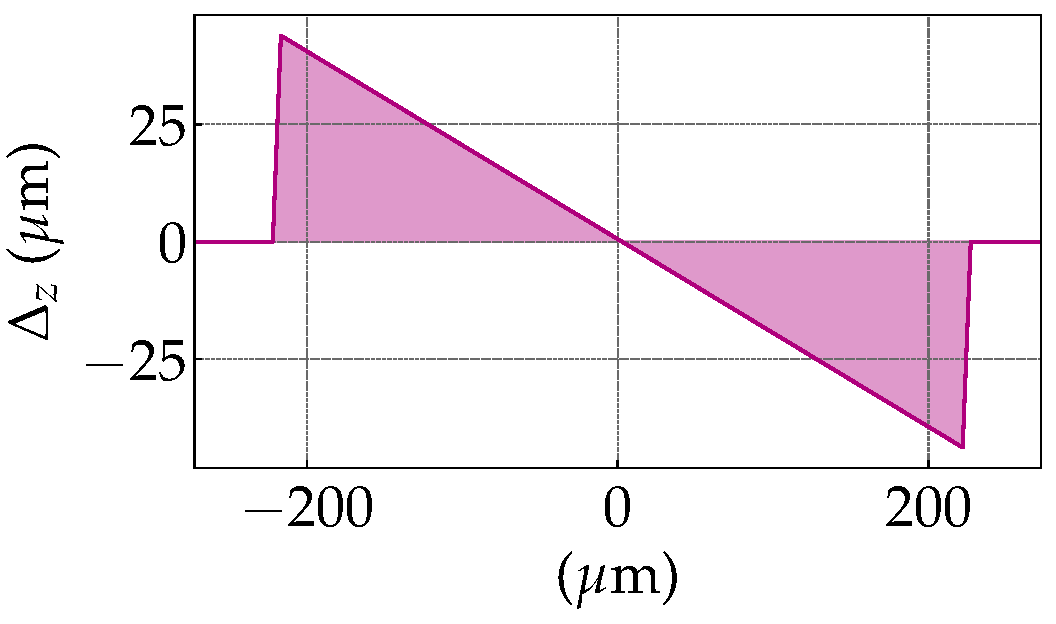
\includegraphics[height=3.cm]{figures/ch04/Be50um_lens_lateral_offset.pdf}}\hspace{0.1cm}
        \subfloat[radiography]{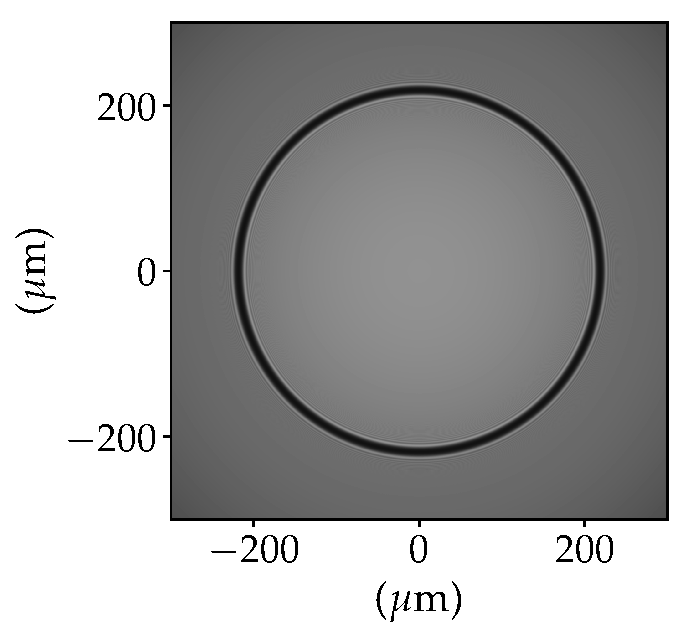
\includegraphics[height=3.4cm]{figures/ch04/radio_CRL_ideal_intensity_intensity_2D.pdf}}\hspace{0.1cm}
        \subfloat[PSF]{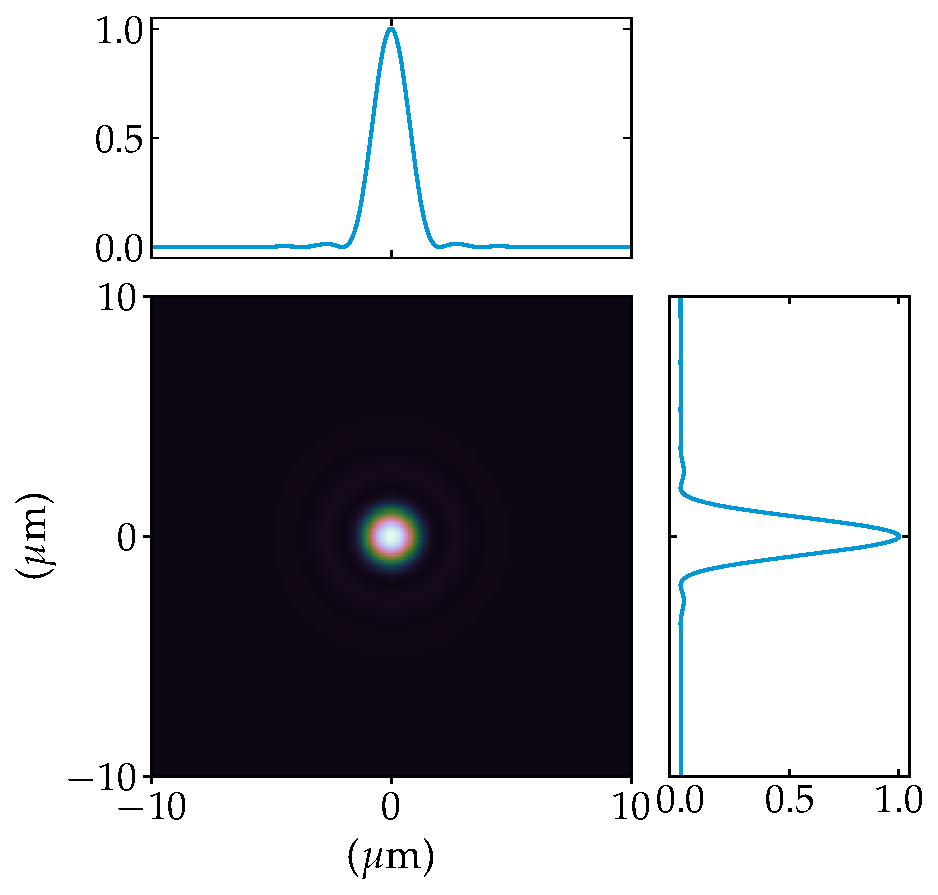
\includegraphics[height=5cm]{figures/ch04/cst_CRL_ideal_intensity_intensity_2D.pdf}}\hspace{0.1cm}
        \subfloat[vertical caustics]{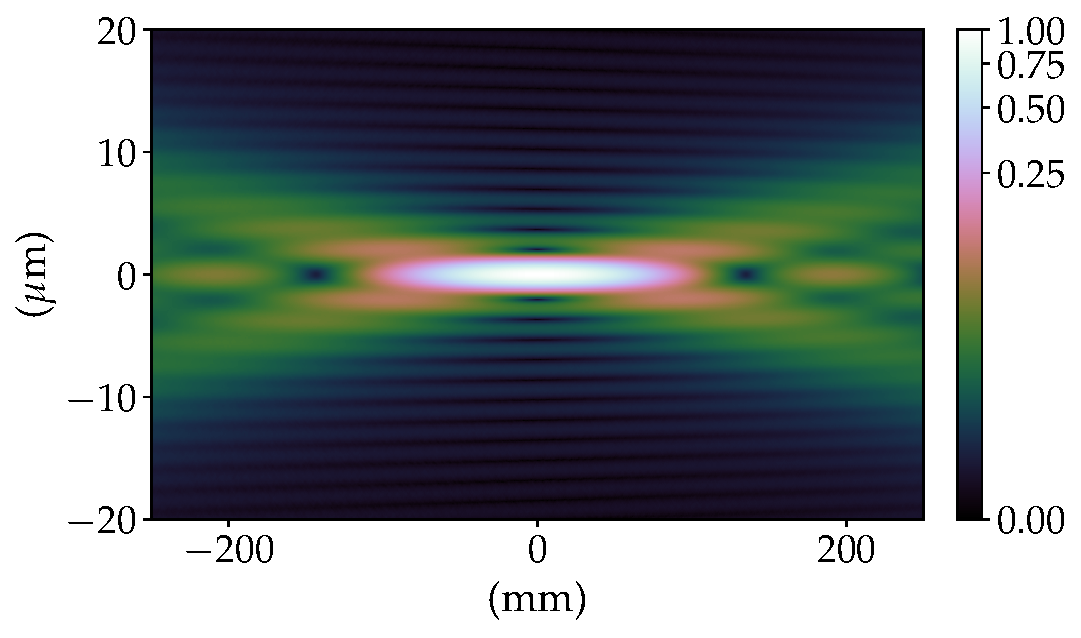
\includegraphics[height=3.5cm]{figures/ch04/cst_CRL_ideal_intensity_cstc_Y_cstc_2D.pdf}}
\end{figure}
\end{document}